% Main file for the GREIT Algorithm
% $Id$
\documentclass[12pt]{iopart}
\usepackage{graphicx}
 \usepackage{amssymb}
 \usepackage{amsbsy}
\newcommand{\vB}{\mbox{$\mathbf{v}$}}
\newcommand{\xB}{\mbox{$\mathbf{x}$}}
\newcommand{\xH}{\mbox{$\mathbf{\hat x}$}}
\newcommand{\xT}{\mbox{$\mathbf{\tilde x}$}}
\newcommand{\XT}{\mbox{$\mathbf{\tilde X}$}}
\newcommand{\nB}{\mbox{$\mathbf{n}$}}
\newcommand{\yB}{\mbox{$\mathbf{y}$}}
\newcommand{\wB}{\mbox{$\mathbf{w}$}}
\newcommand{\AB}{\mbox{$\mathbf{A}$}}
\newcommand{\BB}{\mbox{$\mathbf{B}$}}
\newcommand{\RB}{\mbox{$\mathbf{R}$}}
\newcommand{\IB}{\mbox{$\mathbf{I}$}}
\newcommand{\JB}{\mbox{$\mathbf{J}$}}
\renewcommand{\PB}{\mbox{$\mathbf{P}$}}
\newcommand{\VB}{\mbox{$\mathbf{V}$}}
\newcommand{\WB}{\mbox{$\mathbf{W}$}}
\newcommand{\XB}{\mbox{$\mathbf{X}$}}
\newcommand{\YB}{\mbox{$\mathbf{Y}$}}
% Use boldsymbol when using amssymb
 \newcommand{\SG}{\mbox{${\boldsymbol \Sigma}$}}
 \newcommand{\TG}{\mbox{${\boldsymbol \Theta}$}}
 \newcommand{\sG}{\mbox{${\boldsymbol \sigma}$}}
%\newcommand{\SG}{\mbox{${\mathbf \Sigma}$}}
%\newcommand{\TG}{\mbox{${\mathbf \Theta}$}}
%\newcommand{\sG}{\mbox{${\mathbf \sigma}$}}
\newcommand{\SNR}{\mbox{\small $\mathrm{SNR }$}}
\newcommand{\NF}{\mbox{\small $\mathrm{NF }$}}
\newcommand{\EIT}{\mbox{\small $\mathit{EIT }$}}
\begin{document}

\title[GREIT: linear EIT image reconstruction]{%
GREIT: a unified approach to 2D linear EIT reconstruction of
       lung images
}
%{\small \tt DRAFT: $Date$}

\author{Andy Adler$^{1}$,
        John H. Arnold$^{2}$,
        Richard Bayford$^{3}$,
        Andrea Borsic$^{4}$,
        Brian Brown$^{5}$,
        Paul Dixon$^{6}$,
        Theo J.C. Faes$^{7}$,
        In\'ez Frerichs$^{8}$,
        Herv\'e Gagnon$^{9}$,
        Yvo G\"arber$^{10}$,
        Bart\l{}omiej Grychtol$^{11}$, 
        G\"unter Hahn$^{12}$,
        William R B Lionheart$^{13}$,
        Anjum Malik$^{14}$,
        Robert P. Patterson$^{15}$,
        Janet Stocks$^{16}$,
        Andrew Tizzard$^{3}$,
        Norbert Weiler$^{8}$,
        Gerhard K. Wolf$^{2}$%
       }

\address{ $^{1}$Systems and Computer Engineering,
                Carleton University, Ottawa, Canada}
\address{ $^{2}$Division of Critical Care Medicine, Department of Anesthesia,
                Children's Hospital Boston, Harvard Medical School,
                Boston, MA, USA}
\address{ $^{3}$Department of Natural Sciences,
                Middlesex University, London, UK}
\address{ $^{4}$School of Engineering, 
                Dartmouth College, Hanover, NH, USA}
\address{ $^{5}$Medical Physics, University of Sheffield, UK}
\address{ $^{6}$Cardinal Health Care, London, UK}
\address{ $^{7}$Department of Physics and Medical Technology,
                V.U. university medical center, Amsterdam, Netherlands}
\address{ $^{8}$Department of Anaesthesiology and Intensive Care Medicine,
                University of Schleswig-Holstein, Kiel, Germany}
\address{ $^{9}$D\'epartement de g\'enie \'electrique,
                \'Ecole Polytechnique de Montr\'eal, Canada}
\address{$^{10}$Dr\"ager Medical, L\"ubeck, Germany}
\address{$^{11}$University of Strathclyde, Glasgow, UK}
\address{$^{12}$Department of Anaesthesiological Research,
                University of G\"ottingen, Germany}
\address{$^{13}$School of Mathematics, University of Manchester, UK}
\address{$^{14}$Maltron International, Rayleigh, UK}
\address{$^{15}$Department of Biomedical Engineering,
                University of Minnesota, Minneapolis, MN, USA}
\address{$^{16}$Institute of Child Health,
                University College London, UK}



\begin{abstract}
Electrical Impedance Tomography (EIT) is an attractive method
for clinically monitoring patients during mechanical ventilation,
because it can provide a non-invasive continuous image of pulmonary
impedance which indicates the distribution of ventilation. 
However, most clinical and physiological research in lung EIT
is done using older and proprietary algorithms; this is
an obstacle to interpretation of EIT images because the
reconstructed images are not well characterized.
To address this issue, we are developing a
consensus linear reconstruction algorithm for lung EIT,
called GREIT (Graz consensus Reconstruction algorithm for EIT).
This paper describes the unified approach to 
linear image reconstruction developed for GREIT,
and methods of developing and testing the algorithm.
The framework for the linear reconstruction algorithm
consists of:
1) detailed finite element models of a representative
 adult and neonatal thorax;
2) consensus on the performance figures of merit for
 EIT image reconstruction;
and
3) a systematic approach to optimize a linear reconstruction
 matrix to desired performance measures.
Consensus figures of merit, in order of importance, are:
a) uniform amplitude response,
b) small and uniform position error,
c) small ringing artefacts,
d) uniform resolution,
e) limited shape deformation, and
f) high resolution.
Such figures of merit must be attained 
while maintaining
small noise amplification and
small sensitivity to electrode and boundary movement.
This approach represents the consensus of a large and representative
group of experts in EIT algorithm design and clinical
applications for pulmonary monitoring.
All software and data to implement and test the algorithm has been
made available under an open source license which allows free
research and commercial use. These tools will be used in
the clinical and experimental validation stage of GREIT development.
\end{abstract}

\noindent{\it Keywords\/}:
Electrical Impedance Tomography,
Lung Function Imaging,
Image Reconstruction,

\section{Introduction}
Electrical Impedance Tomography (EIT) measures conductivity
changes within a body, by measuring the voltages at electrodes
on the body surface caused when a number of different
currents are passed through the body.
One of the most promising
applications of EIT is for description of physiologic events
in the thorax, since the thorax contains several
organs which undergo large changes in conductivity
during normal functioning. Indeed, lung function measurement
was among the first physiological applications of this technology
 (Barber and Brown 1984).
%Some imaging modalities can measure ventilation,
%such as MRI (with hyperpolarized He) and PET. However, commonly
%used imaging modalities (radiography, CT, MRI) do not assess
%ventilation directly.
%EIT is unique in that it
%is able to non-invasively and continuously monitor the distribution of 
%ventilation.
EIT is unique in that it is able to non-invasively
measure chest impedance to give a continuous
image of the distribution of ventilation.
Based on these advantages, there is significant
interest in EIT to 
monitor patients with respiratory compromise
(Frerichs \etal 2003, Victorino \etal 2004, Wolf \etal 2007).

One limitation is that most clinical and physiological research
on lung EIT is being done using proprietary variants of
older image reconstruction algorithms, such as the backprojection
algorithm as implemented
in the Sheffield (Brown and Seagar 1987)
or G\"ottingen (Hahn \etal 2002) EIT systems.
The algorithms, although very successful for the time,
   do not incorporate advances that have been made over the last
   20 years.
The reconstructed images show
   spatial non-uniformity in image amplitude, position
   and resolution, which make interpretation of regional
   ventilation difficult and error prone.
For example, because of position errors,
changes near the skin can appear as contrasts in the lung regions.
Many other approaches to the reconstruction of EIT images have been
proposed, incorporating many advances (Lionheart, 2004);
however, such approaches
have not been widely used clinically and experimentally
because there was a lack of an agreement on which
approaches were best (and how they could be combined).

To address this issue, we are developing a
consensus linear reconstruction algorithm for lung EIT,
called GREIT (Graz consensus Reconstruction algorithm for EIT),
since early discussions took place at the 2007 ICEBI conference
in Graz, Austria. Our aim is to develop a standard which
has broad agreement from experts in the mathematical,
engineering, physiological, and clinical EIT communities.
Such an approach is feasible because there is general
consensus amongst experts in lung EIT applications on
the ``ingredients'' that should
be part of a robust and high performance linear algorithm
for 2D EIT of the lungs.
This paper describes the unified approach to 
linear image reconstruction developed for GREIT,
and the tools and evaluation methodology for
clinical and experimental testing of the algorithm.

The current work is limited to the reconstruction algorithm.
At this stage, we do not propose calibration tests, data
 formats or phantoms, standards
for image interpretation or EIT based lung parameters; 
we do not feel there is sufficient experience yet to reach
consensus in these areas.
It is important to clarify that there is no financial
goal to the development of this algorithm.
All developed algorithms, software
models and simulation and experimental test data used
in this algorithm have been
made available under an open source license as part of
the open source EIDORS distribution (Adler and Lionheart 2006);
this license permits
royalty free use in both research and commercial applications.
Additionally, due to space constraints in this paper, only a
limited set of results could be included. The complete
algorithms, results, and source data are available on the 
internet at \verb+eidors.org/GREIT+.



The following specifications have been defined for GREIT:
\begin{itemize}
\item
 single ring electrode
configurations with Sheffield-type EIT systems, using
      adjacent current injection and measurement.
\item
 linear (i.e. real-time) reconstruction of a 2D conductivity
change image, based on a 3D forward model.
\item
 quantitative difference reconstructions for which units can
  be assigned to EIT images.
\item
 reconstruction onto 
      a $32\times 32$ pixel array
      for a single ring of $16$, $12$ and $8$ 
      electrodes, for the shapes:
   a) neonatal chest, 
   b) male and female adult chest, and
   c) cylindrical tank shape.
\end{itemize}

These specifications represent, in our opinion, the limits
to areas sufficiently well understood in the EIT community
to reach consensus. We do not suggest that such limits are ideal;
in fact, we actively encourage work to overcome them, 
such as the single ring placement of electrodes and the consequent
lack of 3D image information. 

\section{Methods: performance figures of merit}
\label{sec:figmerit}

In this section, we elaborate a set of criteria which 
characterize the performance of an ideal reconstruction
algorithm. Clearly, there is an inherent trade-off between
the criteria, such that it is not possible to 
simultaneously optimize all measures. Instead, we proceed
as follows. First, we establish the desired performance measures
of an ideal algorithm; subsequently, 
we describe a unified methodology to calculate a reconstruction
matrix which is an optimized compromise of criteria
weighted by the consensus importance of each.  

We consider an EIT system using the following notation.
Using $n_E$ electrodes,  $n_E$ current stimulation
patterns are sequentially applied and $n_V$ differential voltage 
measurements are made in parallel for each stimulation.
 For an adjacent drive
EIT system, voltages are typically not measured at driven
electrodes, and $n_V = n_E - 3$.  Each data frame measures
a vector, $\vB\in\mathbb{R}^{n_M}$, of $n_M= n_E n_V$ data points
(some of which are redundant if the medium is not changing).
Difference EIT calculates difference data $\yB$, ($[\yB]_i =
[\vB]_i - [\vB_r]_i$); or the normalized difference data $[\yB]_i
= ([\vB]_i - [\vB_r]_i)/[\vB_r]_i)$, where $\vB_r$ is a reference
set of measurements corresponding to the background conductivity
distribution, $\sG_r$. To improve its precision,
$\vB_r$ is typically averaged over many data frames; 
such ensemble averaging reduces random noise, and we
 assume that $\vB_r$ is noise free.



\begin{figure}[bhtp]
\begin{center}
\includegraphics[width=0.8\textwidth,
                 bb=0.0in 1.7in 10in 6.0in,page=1]
                {figures/fig-perf-params.pdf}
\caption{ \label{fig:PerfFigures}
Performance figures of merit for evaluation of GREIT images.
Based on a reconstructed image ($\xH$, {\em left}),
an image ($\xH_q$, {\em centre})
is constructed of all image pixels which exceed
 $\frac{1}{4}$ the maximum amplitude. From these images,
figures of merit at {\em right} are calculated as described.
}
\end{center}
\end{figure}

An outline of the calculation of performance figures
of merit is given in Fig.\ \ref{fig:PerfFigures}.
Given a vector of EIT difference or normalized difference
data, $\yB$ (length $n_E n_V$), we calculate a 
reconstructed EIT image $\xH = \RB \yB$ based on
an EIT linear reconstruction algorithm represented as
a matrix $\RB$. $\xH$ is a column vector representing
the $32\times 32$ pixel grid of the images.

We define figures of merit based on small ``point''
conductivity changes, where small indicates a diameter
of less than 5\% of the medium diameter, and thus
much smaller than the inherent resolution of EIT with
16 electrodes.
To evaluate this image, we first calculate
a $\frac{1}{4}$--amplitude set, $\xH_q$, which
contains all image pixels $[\xH]_i$ greater
than $\frac{1}{4}$ of the maximum amplitude:
\begin{equation}
[\xH_q]_i = \left\{ \begin{array}{ll}
    1 & \mbox{if~} [\xH]_i  \geq \mbox{$ \frac{1}{4}\mathop{max}(\xH)$ } \\
    0 & \mbox{otherwise}.
\end{array} \right.
\end{equation}
For targets
with a conductivity decrease, the definition
of the $\frac{1}{4}$--amplitude set is inverted.
A threshold of $\frac{1}{4}$ represents a compromise
which detects most of the visually significant effects;
however, the exact value of the threshold has little effect on
the final algorithm parameters.
The centre of gravity (CoG) of $\xH$ and $\xH_q$ are
calculated, and the distance from the CoG to the 
medium centre is then calculated, as $r_t$ and $r_q$
respectively.

Based on images of point targets, we define the following
figures of merit:

\begin{itemize}

\item
{\bf Amplitude Response (AR)}
measures the ratio of image pixel amplitudes in the
target to that in the reconstructed image.
For a spherical target of volume $V_t$ in the electrode
plane with
conductivity $\sigma_t$ in a body of homogeneous reference
conductivity $\sigma_r$
\begin{equation}
\mathrm{AR} =  \frac{
    \sum_k [\xH]_k
  }{
    V_t \frac{\Delta\sigma}{\sigma_r}
  }
\end{equation}
where $\Delta\sigma = \sigma_t - \sigma_r$,

\hspace{5mm}
AR allows units to be assigned to the 
reconstructed conductivities. For this, we 
require that reconstruction matrices, $\RB$, be
scaled such that AR$=1$ for 
a small spherical target with
 $\Delta\sigma/\sigma_r \approx 1$
in the centre of the body.
With this normalization, reconstructed EIT images have
units as follows:
   \begin{itemize}
   \item {\em Normalized Difference EIT:}
in this case, measurements $\yB$ are unitless,
and the EIT image will be in units of fractional conductivity
change, $\Delta\sigma/\sigma_r$.
   \item {\em Difference EIT:}
in this case, measurements $\yB$ must be in units of
transfer conductance ($\Omega^{-1}$), and the EIT image
will be in units of conductivity change (in $\Omega^{-1}\cdot$m)
scaled by the ratio or the measurement geometry to
the FEM geometry.
% for a box of A, L, admittance = A sigma / L
% if we scale it by s, admittance = s^2 sigma / sL = s admittance_0
% so admittance scales by the model to real scale ratio.
   \end{itemize}


\hspace{5mm}
{\em Desired behaviour:}
AR should be constant for any target position. We consider
constant
AR to be the most important figure of merit, since, without
constant amplitude response, the same volume of air in different parts
of the lung will contribute differently to the image, introducing
serious difficulties in image interpretation.

\item
{\bf Position Error (PE):}
measures the extent to which reconstructed images faithfully
represent the position of the image target. Based on the
target position, $r_t$, and the CoG of $\xH_q$, $r_q$, we define:
\begin{equation}
\mathrm{PE} = r_t - r_q
\end{equation}
where positive values of PE indicate reconstructed images
``pushed'' to the medium centre. This measure is similar
to that of Adler and Guardo (1996).

\hspace{5mm}
{\em Desired behaviour:}
PE should be small and show small variability for
targets at different radial positions. We consider
small and constant PE to be the second most important
figure of merit. If PE is variable, interpretation
of a distribution of air in the lungs becomes unreliable.
Sheffield backprojection has large PE near the
electrodes, and this has resulted in cases where changes at
the electrodes are misinterpreted as being inside the body.

\item
{\bf Resolution (RES):}
measures the size of reconstructed targets as a fraction
of the medium; this is
equivalent to a measure of point spread function (PSF) size.
\begin{equation}
\mathrm{RES} = \sqrt{
 \frac{ A_q }
      { A_0 }
 }
\end{equation}
where $A_q =  \sum_k [\xH_q]_k$, the number
of pixels in $\xH_q$ and 
$A_0$ is the area (in pixels) of
the entire reconstructed medium. The square root is used 
so that RES measures radius ratios rather than area ratios.
This measure is modelled on the one proposed by
Wheeler \etal (2002).

\hspace{5mm}
{\em Desired behaviour:}
RES should be uniform and small, in order to 
more accurately represent shape of the target conductivity
distribution. We consider uniformity of RES to be the
fourth most important figure of merit, but small size
of RES to be less important (sixth). A non-uniform
RES can result in an incorrect reconstructed 
position of a larger target. Low RES serves primarily
to distinguish nearby targets. Since EIT is understood to
be a low resolution medium, this application is less important.

\item
{\bf Shape Deformation (SD):}
Reconstruction algorithms typically create circular
images for targets in the centre, but often display 
strangely shaped artefacts for targets near the medium
boundary. Backprojection tends to show ``streak''
artefacts in this case.
SD measures the fraction of the reconstructed
$\frac{1}{4}$--Amplitude set which does not
fit within a circle of equal area.
\begin{equation}
\mathrm{SD} = \sum_{k\not\in C} [\xH_q]_k / 
              \sum_{k} [\xH_q]_k
\end{equation}
where $C$ is a circle centred at the CoG of $\xH_q$
with an equivalent area to $A_q$. This figure
is similar to that of Oh \etal (2007).

\hspace{5mm}
{\em Desired behaviour:}
SD should be low and uniform. Large SD may result in
incorrect interpretation of images, although this
effect is less important than other artefacts. We 
consider SD to be the fifth most important figure 
of merit.

\item
{\bf Ringing (RNG):}
measures whether reconstructed images show
areas of opposite sign surrounding the main 
reconstructed target area. Fig. \ref{fig:PerfFigures}
shows an arc of ringing around the image centre.
Ringing is typical of linear filters; for second-order
systems the effect may also be called ``overshoot''.
RNG measures the ratio of image amplitude of
the opposite sign outside circle $C$ to image
amplitude within $C$.
\begin{equation}
\mathrm{RNG} =
\left(
        \sum_{k\not\in C \& [\xH]_i < 0} [\xH]_k 
\right)
/ 
\left(
        \sum_{k\in C}                    [\xH]_k 
\right)
\end{equation}

\hspace{5mm}
{\em Desired behaviour:}
RNG should be low and uniform. Overshoot may
easily result in incorrect interpretation. For
example, the negative ringing between non-conductive
lungs will produce a conductive pattern which 
may be misinterpreted as a heart.
We consider RNG to be the third most important figure 
of merit.

\begin{figure}[bhtp]
\begin{center}
\includegraphics[width=0.4\textwidth,
                 bb=1.5in 2.0in 6.5in 6.0in,page=1]
                {figures/fig-noise-fig.pdf}
\caption{ \label{fig:noise_fig}
Schematic representation of the Noise Figure (NF)
parameter. NF represents the amplification of noise through
the reconstruction process as the ratio of SNR$_x$ to SNR$_y$.
}
\end{center}
\end{figure}

\item
{\bf Noise Amplification (NF):}
measures the extent to which random
measurement noise is amplified
in the reconstructed images. Noise amplification
is measured by the noise figure (NF) as
illustrated in Fig. \ref{fig:noise_fig}, 
based on the definition by Adler and Guardo (1996).
The NF is the ratio of the output to input
 signal to noise ratio (SNR) for a filter.
We define SNR~=~%
$\frac{
   \mbox{mean \em signal}
      }{
   \mbox{std \em noise}
     }
$ 
in terms of image amplitude,
rather than in terms of image energy, since linear
image reconstruction tends to conserve  amplitude
rather than energy. Thus
\begin{equation}
\mathrm{NF} = \frac{
   E[ \mathop{mean}~\xH_t ] 
         /
   E[ \mathop{std}~\xH_n ]
}{
   E[ \mathop{mean}~\yB_t ] 
         /
   E[ \mathop{std}~\yB_n ]
}
\end{equation}
For regularized algorithms, the value of NF is normally
set by selection of the value of 
a hyperparameter. For GREIT, the value of NF is set by the weighting
associated with the training noise. There is an inherent
trade-off between good noise performance and fidelity to
the other figures of merit.

\hspace{5mm}
{\em Desired behaviour:}
NF should be low, and, ideally, should be tuned to the noise
level present in the EIT hardware used.
Several studies have looked into strategies to select
appropriate noise performance (eg. Graham and Adler 2006).
At this time, we do not have consensus on the best
way to choose NF. Instead, we note that noise performance
of Sheffield Backprojection (NF=$0.5$ in the medium center)
has generally been considered to be satisfactory.
Therefore, as an interim measure, we recommend NF=$0.5$
for GREIT algorithms.

\end{itemize}

\section{Methods: Reconstruction algorithm framework}

This section describes the GREIT framework to calculate
a linear image reconstruction matrix which is optimized
to a set of performance requirements. This approach
is based on experience with a large number of 
linear regularized EIT reconstruction approaches
(such as
Adler and Guardo 1996,
Adler and Lionheart 2006,
Barber and Brown 1988,
Cheney \etal 1990,
Cohen-Bacrie \etal 1997,
Polydorides and Lionheart 2002,
Soleimani \etal 2006,
Vauhkonen \etal 1998).
The key difference is that this framework
is based on a set of performance requirements, whereas
previous reconstruction algorithms are based directly on
the underlying mathematical models and do not express
the performance requirements explicitly.
The value of this approach is that it allows
these performance requirements (established in our case
via consensus) to be directly encoded into the
reconstruction algorithm.

The body under investigation is modelled using a finite element
model (FEM) which discretizes the conductivity onto $n_N$
piecewise smooth elements, represented by a vector
$\sG\in\mathbb{R}^{n_N}$ (To clarify use of symbols,
$\sG$ represents a vector conductivity distribution, while
$\sigma$ is the standard deviation).
Again, difference EIT calculates a vector of
conductivity change, $\xB = \sG - \sG_r$ between the present,
$\sG$, and the reference, $\sG_r$,
conductivity distributions.

Image reconstruction in EIT is a non-linear problem; however,
linearized approximations have proved to be very useful.
This is largely because the noise levels present in clinical
and experimental EIT data are sufficiently large
to prevent stable results with iterative algorithms.
Linear algorithms also have the benefit of producing
images in which the effects
of data artefacts can be more readily identified. Finally,
linear reconstruction can be implemented as a fast matrix
multiplication. We represent linear EIT image reconstruction
as a matrix, $\RB\in\mathbb{R}^{n_N\times n_M}$ which
maps measurements $\yB$ to a reconstructed image $\xH$:
\begin{equation} 
\label{reconst_eqn}
   \xH = \RB \yB
\end{equation} 
 

\subsection{Sheffield Backprojection}

The backprojection algorithm was developed by 
Barber and Brown (1984) for the original 
Sheffield EIT system, and  has seen numerous 
variants and improvements (Barber, 1989). While the original
technique was based on an analogy to the backprojection
algorithm for CT, this model was clearly inadequate, because
electric current propagates diffusely, and thus differently
to X-ray photons. Therefore, improvements
were developed to the backprojection algorithm
(e.g.\ Barber and Brown 1988). Such strategies
can be shown to regularize the reconstructed images.
A good mathematical characterization is given by
Santosa and Vogelius (1990).

While many variants of Sheffield backprojection exist,
clinical and experimental EIT has largely used only
one: that which was distributed in the
Sheffield Mark I EIT system (Brown and Seagar 1987).
The G\"ottingen Goe MF II EIT system (Hahn \etal 2002)
has also been widely used for such clinical and
experimental work, and uses a very similar reconstruction
algorithm.

This paper compares GREIT to the Sheffield Mark I
backprojection algorithm;
unfortunately, it appears that the exact formulation
of the specific algorithm version of interest has been
lost. To reconstruct it, we proceeded as follows.
Since image reconstruction is linear, there exists
a mapping which can explain the transformation of
measurements into images. We obtained a large set of
measurements, $\yB_k$, and the associated
reconstructed images, $\xH_k$, and formed matrices
$\YB = [ \yB_1, \cdots, \yB_k, \cdots]$ and 
$\XB = [ \xH_1, \cdots, \xH_k, \cdots]$ by concatenation.
The Sheffield backprojection matrix, was
calculated as the least squared fit to
   $\YB \RB_{SBP} = \XB$.
In order to permit testing of EIT data against
this algorithm, it has been made available
online 
\verb$eidors.org/data_contrib/db_backproj_matrix$
under the following license:
``This matrix is copyright DC Barber and BH Brown at
  University of Sheffield. It may be used free of charge
  for research and non-commercial purposes. Commercial
  applications require a license from the University of Sheffield.''


\subsection{One step linear Gauss-Newton solvers}
\label{subsec:OSLGNS}

In this section, we elaborate the
Gauss-Newton (GN) EIT reconstruction approaches,
which have been
widely used in EIT since the late 1980's (Yorkey \etal 1987,
Cheney \etal 1990).
This approach allows use of sophisticated regularized models
of the EIT inverse problem, able to represent this
solution as a linear reconstruction matrix, which can then allow
rapid, real-time imaging.
For small variations around the reference
conductivity $\sG_r$, the relationship between $\xB$ and $\yB$ can
be linearized (giving the difference EIT forward model):
\begin{equation}\label{FM}
\yB=\JB\xB+\nB
\end{equation}
where
$\JB\in\mathbb{R}^{n_M\times n_N}$ is the Jacobian or sensitivity
matrix and $\nB\in\mathbb{R}^{n_M}$ is the measurement noise, which is
assumed to be uncorrelated white Gaussian. $\JB$ is calculated from
the FEM as
$[\JB]_{ij}=\left.
     \frac{\partial[\yB]_i}{\partial[\xB]_j}
          \right|_{\sG_r}$,
and depends on the FEM, current injection patterns, the reference
conductivity, and the electrode models. This system is
underdetermined since $n_N > n_M$. 
Regularization techniques are required
in order to calculate a conductivity change
estimate, $\xH$, which is both
faithful to the measurements, $\yB$, and to
{\em a priori} constraints on a ``reasonable'' image.

The GN inverse problem seeks to
calculate a solution, $\xH$, to the EIT inverse problem
in terms of a generalized Tikhonov regularization 
expressed as the minimum of a sum of quadratic norms
\begin{equation}\label{IM}
 \|\yB-\JB\xH\|_{\Sigma_n^{-1}}^2 +
 \|\xB-\xB^\circ\|_{\Sigma_x^{-1}}^2
\end{equation}
where $\xB^\circ$ represents the expected value of element
conductivity changes, which is zero for  difference EIT.
$\SG_n\in\mathbb{R}^{n_M\times n_M}$ is
 the covariance matrix of the measurement noise $\nB$. Since
$\nB$ is uncorrelated, $\SG_n$ is a diagonal matrix with
$[\SG_n]_{i,i}=\sigma_i^2$, where $\sigma_i^2$ is the noise variance at
measurement $i$. $\SG_x\in\mathbb{R}^{n_N\times
n_N}$ is the expected image covariance.

It is worth noting that many other regularized approaches
to EIT have been used, such as the
TSVD (truncated singular value decomposition; Bayford \etal 2008)
and
SIRT (simultaneous iterative reconstruction technique; Hahn \etal 2006).
All linear approaches are structurally similar; however
the formulation in (\ref{IM}) is more general
as it explicitly exposes the selection of image reconstruction
parameters.



Typically,  covariance matrices
$\SG_n$ and $\SG_x$ are not calculated directly, but
are modelled heuristically from {\em a priori}
considerations as 
 $\VB = \sigma_n^{2}\SG_n$
 and
 $\PB = \sigma_x^{2}\SG_x$,
where $\sigma_n$ is the average measurement noise amplitude and
$\sigma_x$ is the {\em a priori} amplitude of conductivity change.
$\VB$ models the measurement accuracy. For uncorrelated noise,
each diagonal element is proportional to the signal to noise
ratio. For difference EIT with identical channels, $\VB=\IB$. The
regularization matrix $\PB$ may be understood to model the
likelihood of image elements and their interactions.

By solving (\ref{IM}), a linearized, one-step inverse solution is
obtained as
\begin{eqnarray}\label{GN_solution}
\xH&=&\left(
    \JB^T \frac{1}{\sigma_n^2} \VB^{-1} \JB 
     +
    \frac{1}{\sigma_x^2} \PB^{-1}
    \right)^{-1}
    \JB^T \frac{1}{\sigma_n^2}\VB^{-1}\yB
\nonumber \\
   &=&\left(
    \JB^T \VB^{-1} \JB + \lambda^2 \PB^{-1}
    \right)^{-1}
    \JB^T \VB^{-1} \yB
\end{eqnarray}
where parameter  $\lambda=\sigma_n/\sigma_x$ is
often called the ``regularization hyperparameter'' and
controls the trade-off
between resolution and noise attenuation in the reconstructed
image.
The matrix,
$\RB=\left(\JB^T\VB^{-1}\JB+\lambda^2\PB^{-1}\right)^{-1}\JB^T\VB^{-1}$
is the linear, one-step inverse.
In (\ref{GN_solution}), the term in the inverse is of size
$n_N\times n_N$. To save computational time, and improve inverse
accuracy and stability, matrix $\RB$ may be rewritten 
using the {\em data form}, or {\em Wiener filter form} as:
\begin{equation}\label{opti_sol}
 \RB =\PB\JB^T
    \left(
       \JB\PB\JB^T+\lambda^2\VB
   \right)^{-1}
\end{equation}
In (\ref{opti_sol}), the size of the term in the
inverse is reduced to $n_M\times n_M$.

If image elements are assumed to be independent with identical
expected magnitude, $\PB$ becomes an identity matrix $\IB$ and
(\ref{GN_solution}) uses zeroth-order Tikhonov regularization. For
EIT, such solutions tend to push reconstructed noise toward the
boundary, since the measured data are much more sensitive to
boundary image elements. Instead, $\PB$ may be scaled with the
sensitivity of each element, so that each diagonal element $i$ 
$[\PB^{-1}]_{i,i} = \left[ \JB^T \JB
\right]_{i,i}^p$. This is the NOSER prior of Cheney \etal (1990)
for an exponent $p=1$. Many other prior matrices have been
proposed: to model image smoothness as a penalty for non-smooth
image regions, $\PB$ may be set to the discrete Laplacian filter
(Vauhkonen \etal 1998), a discrete high pass Gaussian filter (Adler
and Guardo 1996), or based on variance uniformization
constraints (Cohen-Bacrie \etal 1997).
In this paper, we compare results from the GREIT approach
with those of GN image reconstruction using the NOSER prior,
$\PB$ with $p=1.0$.  The NOSER algorithm is 
representative of a broad group of structurally similar 
algorithms that have been widely implemented in EIT;
it is generally understood to perform well.


\subsection{GREIT image reconstruction approach}

In this section, we elaborate the GREIT procedure
from which the reconstruction matrix, $\RB$ is
calculated.  The procedure depends on definition
of a forward model, a noise model, and
desired performance metrics.

\subsubsection{Forward model}

A forward model allows calculation of EIT
 measurement
data $\yB^{(k)}$ from a conductivity change distribution $\xB^{(k)}$.
The model represents the details of the body geometry,
the electrode size and contact impedance, and the reference
conductivity, $\sG_r$, around which conductivity changes occur.
In this paper, the forward problem is solved using a
3D FEM using the complete electrode model
(Cheng \etal 1989). However, it is worth noting that 
any forward model, physical or numerical, is suitable
for this procedure.

One other requirement for the forward problem model is
an estimate of the amplitude of conductivity changes $\xB^{(k)}$
encountered in the modelled EIT application. Based on the
forward model, conductivity changes, $\xB$, result in
a measurement variance
$\sigma_{\yB}^2 = \mathrm{var}~\yB = E[ \| \yB \|^2 ]$. 
The mean $\yB$ is assumed to be zero, which implies
that positive and negative conductivity changes are
equally likely. This assumption is reasonable for a 
general purpose EIT reconstruction algorithm, although
specific EIT applications may not match it exactly.
For lung images, we may calculate $\sigma_{\yB}^2$ using
either a simulation model
of the amplitude of conductivity changes due
to breathing, or from a sample of EIT measurements 
in representative applications.

\subsubsection{Noise model}

A noise model allows calculation of representative 
noise (or undesired signal) samples in EIT measurements.
For GREIT, we consider two sources of noise:
electronic measurement noise, and
electrode movement artefacts. In general, for each
source of noise $n_s$, we have noise samples $\yB^{(k)}_{n_s}$,
and an estimate of the noise amplitude variance
 $\sigma_{n_s}^2 = \mathrm{var}~\yB_{n_s} = E[ \| \yB_{n_s} \|^2 ]$. 
The mean noise is assumed to be zero in this formulation;
if necessary, a non-zero noise mean should be accounted for
by pre-processing of EIT measurements.
Note that for normalized difference EIT,
noise samples are normalized by the
reference measurements by $[\yB]_i = [\nB ]_i / [\vB_r]_i$.

{\em Electronic measurement noise}
is typically modelled to be uniform and Gaussian in EIT
image reconstruction. This assumption is reasonable for
a generic GREIT algorithm designed for general EIT reconstruction.
However, for a specific EIT system, measurement noise
is a function of the EIT hardware and patient
connection. If different gain settings are used for each
channel, these settings will alter the noise. Calibrated
measurements of EIT noise show that it is non-Gaussian and
varies between channels (Hahn \etal 2008).
 We suggest GREIT algorithms
be tuned to the hardware implementation. This may be 
implemented using a calibration protocol before the 
start of measurements, or by integrating a model of 
the hardware imperfections into the forward model
(Hartinger \etal 2007).

{\em Electrode movement artefacts}
occur when the electrodes move, either with posture change
or with chest movements due to breathing. Several reports
have demonstrated the significant impact of such movements on
EIT images (Adler \etal 1996, Zhang and Patterson 2005,
Coulombe \etal 2005). In order to reduce the contribution
of such movement on EIT reconstruction, Soleimani \etal
(2006) showed that it is possible to create an
augmented forward model based on both the conductivity change
and electrode movement, which resulted in reduced movement 
artefacts in the reconstructed images. In order
to use this capability in GREIT, we specify that a
set of ``noise'' measurements due to electrode movement 
be incorporated. This is currently implemented from
deformations of the FEM (G\'omez-Laberge and Adler 2008),
but may be based on a calibration protocol in an
implemented system.

\begin{figure}[bhtp]
\begin{center}
\includegraphics[width=0.6\textwidth,
                 bb=0.0in 1.7in 10in 6.0in,page=1]
                {figures/fig-training-set.pdf}
\caption{ \label{fig:desired_performance}
Training data for GREIT. Two sets of training data are used, based on
conductivity targets and noise or artefact sources. For each type
data, a set of training inputs (EIT measurements) and desired
outputs (reconstructed images) are calculated. Rectangles represents
a matrix in which each column $(k)$ represents training
sample. The circle represents corresponding desired image pattern.
}
\end{center}
\end{figure}

 
\subsubsection{Desired performance metrics.}

Based on the performance metrics defined
in section \ref{sec:figmerit},
we can create training set of ``desired images'', $\xT_t$.
For training set member $(k)$, each image, $\xT_t^{(k)}$,
corresponds to the position of a conductivity target,
$\xB_t^{(k)}$, in the forward model, as illustrated
in Fig.\ \ref{fig:desired_performance}. The desired
image, $\xT_t$, is located at the same centre as the
conductivity target, $\xB_t$. The difference
is that $\xT_t$ is defined to be a circle with a circular
area corresponding to the blurring inherent in EIT,
while $\xB_t$ is essentially a point target. It is this
definition of a larger ``desired image'' which allows
GREIT to achieve a more uniform resolution.
Since most EIT reconstruction algorithms
achieve better resolution near the boundary than in the medium
centre, this definition of $\xT_t$ forces a trade-off
of boundary resolution for a lower resolution that
can be achieved uniformly throughout the image.
Note that it would possible to set
$\xT_t^{(k)} = \xB_t^{(k)}$; however, this would be equivalent to a standard
GN solution without tuning the algorithm to the 
performance metrics.
We recommend, for a 16 electrode
EIT system, that the diameter of $\xT_t$
be 20\% of the medium diameter.
For noise samples, the ``desired image'' is clearly
zero; we wish for noise input to produce no output.

Corresponding to each ``desired image'', is an image
weighting $\wB^{(k)}$ which represents the weight given to 
each pixel in $\xT^{(k)}$. The weighting allows ``tuning''
of the relative importance of the  performance metrics,
as illustrated in Fig. \ref{fig:training_weighting}.
For each desired image, $\xT^{(k)}$, there is an inner
circular zone centred at the target position
where the amplitude is required to be
flat to meet the AR and PE performance metrics.
There is another circular zone outside the boundary
of the specified contrast, where the desired image
is zero, to meet the RNG and SD performance metrics
(illustrated as the circles on Fig. 
\ref{fig:training_weighting} bottom left).
In these zones, $\wB^{(k)}$ is large in order to
provide a substantial penalty for images outside the
specifications. Between the circles we have a 
``transition zone'' in which the reponse gradually
decreases from the specified amplitude to zero.
In the transition zone, $\wB^{(k)}$ is small to allow 
the reconstruction algorithm flexibility to meet the
other specifications. For training data with noise,
$\yB_n^{(k)}$, $\xT^{(k)}=0$, as mentioned above.
For these images, the weighting, $\wB^{(k)}$ is
uniform across the image area. The magnitude
of $\wB^{(k)}$ controls NF and the overall noise
performance of GREIT. A large value of $\wB^{(k)}$ 
results in a large penalty for image noise 
and a low NF, and vice vera.


\begin{figure}[bhtp]
\begin{center}
\includegraphics[width=0.8\textwidth, bb=0.0in 2.7in 10in 7.5in,page=1]{figures/fig-weighting.pdf}
\caption{ \label{fig:training_weighting}
Illustration of the training data and weighting.
{\em left:}   Training target ($\xB_t^{(k)}$)
{\em centre:} Reconstructed image ($\xH^{(k)}$)
{\em right:}  Desired image ($\xT^{(k)}$)
The bottom row shows the image while the top row plots
the amplitude across a row through the centre of the
simulation target. $\xT^{(k)}$ is larger than $\xB^{(k)}$
in order to establish a uniform resolution. The weighting
$\wB^{(k)}$ is illustrated on the image of $\xT^{(k)}$
by two circles. Inside the inner circle and outside the
outer circle, $\wB^{(k)}$ is larger, illustrated by the
small error bars on the upper graph. Between the circles, in
the ``transition zone'', $\wB^{(k)}$ is smaller,
 illustrated by the larger error bars.

}
\end{center}
\end{figure}


Based on the {\em forward model}, {\em noise model},
and {\em desired performance metrics}. we are
able to formulate a set of training data and
define the GREIT reconstruction matrix $\RB_{GR}$
in terms of these data. We can show that
for a linear reconstruction, this approach is 
equivalent to a generalized Tikhonov regularization
(section \ref{subsec:OSLGNS})
in which the prior distributions $\SG_x$ and $\SG_n$
correspond to the selection strategy for
the training data
(section \ref{subsec:training_data}).
The
reconstruction matrix $\RB_{GR}$ which best fits the requirements
may be expressed as minimization of an error $\epsilon^2$
\begin{equation}
\label{GREIT_norm}
\epsilon^2 = \sum_k \| \xT^{(k)} - \RB \yB^{(k)} \|_{(\WB^{(k)})^2}
    = \sum_k \| (\WB^{(k)})^2 (\xT^{(k)} - \RB \yB^{(k)} ) \|^2
\end{equation}
where $\WB^{(k)} = diag( \wB^{(k)})$, is a diagonal matrix representing
the weighting corresponding to each measurement.
 The 2-norm is used as it allows
a linear expression for, and faster computation of, $\RB$;
however, other norms may result in improved performance.

Based on (\ref{GREIT_norm}), we develop an expression
for $\RB = \arg\min~\epsilon^2$, by setting the
matrix derivative of $\epsilon^2$ to zero.
\begin{equation}
\frac{ d\epsilon^2 }{ d\RB_{ij} } =
-2 \sum_k (\xH^{(k)})^T (\WB^{(k)})^2 [\TG]_{i,j} \yB^{(k)}
+2 \sum_k (\yB^{(k)})^T [\TG]_{i,j} (\WB^{(k)})^2 \RB \yB_k
\end{equation}
where $[\TG]_{i,j}$ has a value of $1$ at $(i,j)$
but is zero elsewhere. Based on this expression
\begin{eqnarray}
  \sum_k (\xH^{(k)})^T (\WB^2)^{(k)} [\TG]_{i,j} \yB^{(k)}
 &=&
  \sum_k (\yB^{(k)})^T [\TG]_{i,j} (\WB^2)^{(k)} \RB \yB^{(k)}
\nonumber
\\
  \sum_k [\yB^{(k)}]_j [\wB^{(k)}]_i^2 [\xT^{(k)}]_i 
 &=&
  \sum_l [\RB]_{i,l} \sum_k [\yB^{(k)}]_l [\wB^{(k)}]_i^2 [\yB^{(k)}]_j 
\end{eqnarray}

This expression may be represented as a matrix equation
by defining matrices $\AB$ and $\BB$.
\begin{equation}
\AB = \sum_k (\WB^{(k)})^2 \xT^{(k)} (\yB^{(k)})^T 
\end{equation}
and $\BB$ is the vertical concatenation of $n_N$
($n_M \times n_M$) block matrices $\BB_l$, where
\begin{equation}
\BB_l = \sum_k [\wB^{(k)}]_l^2 \yB^{(k)} (\yB^{(k)})^T 
\end{equation}
Based on these expressions, $\RB_{GR}$ is the
least squares minimizer of the norm 
$\|\AB_{(:)} - \RB_{(:)} \BB\|^2$ where
the notation $(:)$ indicates row concatenation of a matrix.
Thus the GREIT reconstruction matrix, $\RB_{GR}$
is calculated
\begin{equation}
\RB_{(:)}^T = \BB (\BB^T \BB)^{-1} \AB_{(:)}^T
\end{equation}

The calculation of the GREIT reconstruction matrix
may be shown to be equivalent to a scaled generalized
Tikhonov solution of the form of section \ref{subsec:OSLGNS}.
In order to illustrate this equivalence, consider
a GREIT reconstruction algorithm formulated
with uniform weighting $\WB$ for each sample, $k$. For the training set,
$n_T$, training conductivity targets, $\yB_t^{(k)}$, are drawn from
a distribution with covariance $\SG_x$.
For this example, we consider $n_{M_N}$ samples of only the electronic
measurement noise, $\yB_n^{(k)}$, which is modelled as Gaussian,
and samples are drawn from a distribution with 
covariance $\SG_n$. The reconstruction matrix $\RB$ minimizes
the norm
\begin{equation}
\| [ \XT_t, 0 ] - \RB [ \YB_t, \YB_n ] \|_{\WB^2}^2
\end{equation}
where $[\cdot,\cdot]$ represents horizontal
matrix concatenation and
$\YB_t = \frac{1}{n_T}    [ \yB_t^{(1)} \cdots \yB_t^{(n_T)} ]$,
$\XT_t = \frac{1}{n_T}    [ \xT_t^{(1)} \cdots \xT_t^{(n_T)} ]$,
and 
$\YB_n = \frac{1}{n_{M_N}} [ \yB_t^{(1)} \cdots \yB_t^{(n_{M_N})} ]$.
In this case, the matrix $\RB$ which minimizes the norm is 
\begin{eqnarray}
\RB &=& [ \XT_t, 0 ] [\YB_t, \YB_n]^T
     \left( [\YB_t, \YB_n] [\YB_t, \YB_n]^T \right)^{-1}
\nonumber \\
    &=& \XT_t \YB_t^T \left( \YB_t \YB_t^T + \YB_n \YB_n^T \right)^{-1}
\nonumber \\
    &=& \XT_t \YB_t^T \left( \JB \SG_x \JB^T + \SG_n \right)^{-1}
\end{eqnarray}
where samples $\YB_t$ may be approximated from the Jacobian
assuming the body is linear for small targets. This formulation 
has the same generalized Tikhonov regularization 
term as that 
of eqn.\ (\ref{opti_sol}).


\subsection{Selection of training data}
\label{subsec:training_data}

Training data are selected as small, conductivity contrasting
targets spread randomly and uniformly in the plane of 3D model
between electrodes. Vertical offsets above and below the
plane of $0.25\times$diameter of medium are allowed.

The computational cost of calculating $\RB_{GR}$ does
not change dramatically with the size of the training data
set. The size of the matrix to be inverted is fixed at
$n_M \times n_M$. We therefore use a large number of
training samples. The minimum training set 
is much smaller, because, since the model is
linear, the key requirement is that the range of 
$\RB_{GR}$ be adequately represented, and it is limited
to the number of independent measurements,
$\frac{1}{2} n_E \times n_V$ (which, for a 16 electrode
system is 104).

\section{Methods: forward models}

Training data for GREIT requires a forward model which
maps conductivity contrast targets, $\xB_t$, to difference
measurements, $\yB$. Forward models are built using
3D first order tetrahedral finite elements, and
solved using preconditioned linear solvers
(Polydorides and Lionheart 2002).
Finite element models have been developed for four
different geometries: 
male and female adult chests,
a neonatal chest, and
a cylinder. The cylindrical form may be used
for phantom studies, and to image a pig thorax
(which has a roughly circular cross section).
Clearly, it is possible to design optimized
models for a given patient geometry, and this
will offer improved reconstructed images,
% ??? (REFS showing improvement due to accurate models),
with the added complexity of designing
patient specific FEM meshes.
Based on our experience with time-difference
EIT, we feel that the four models provided offer
most of the accuracy of adaptive meshing.

In the design of FEM models of the thorax, the
following issues need to be considered.
\begin{itemize}
\item
{\em Electrode placement:}
Several configurations of electrode types and placement
are currently used. GREIT considers electrodes placed
in a plane at a defined chest height perpendicular to 
the patient long axis. In the most common configuration,
Electrode \#1 is placed on the sternum. Subsequent
electrodes are placed on subject left, spaced equidistantly
around the chest. When viewing the EIT image, electrodes
are numbered clockwise from the top centre, and the subject
is oriented so the feet would point out of the image. Another
common configuration places electrodes \#1 and \#16 on
either side of the sternum, and rotates the remaining 
electrodes accordingly.
%??? Can we reference any publications explaining this?

\hspace{0.5cm}
Electrodes placed at a mid-thoracic level show a 
good approximation of the global lung behaviour
(Yang and Patterson 2007).
There are two main strategies to select the electrode
level.  One practice is to place
electrodes at a defined distance (a few centimeters 
in adults and millimeters in infants)
below the nipple line, although this anatomical
marker is somewhat variable for some female and
larger or older male subjects. 
The other approach is to 
place the electrodes at the level of the
$6^{\rm th} - 7^{\rm th}$ intercostal space at
the parasternal line (which corresponds approximately
to the nipple line). Other vertical placements have
been reported: the $10^{th}$ intercostal space 
(Coulombe \etal 2005), and  
the upper chest at the $3^{\rm rd}$ intercostal space
to measure lung perfusion (Smit \etal 2004).
Placing electrodes too low may result in a large
contribution of mediastinum or abdominal impedance
changes in the center of the EIT image.

\item
{\em Electrode size:}
Electrode size varies between applications. Lung
EIT applications typically
use standard Ag/AgCl ECG electrodes.
For applications with custom EIT electrodes, it is
common to use larger electrodes, in order to decrease
variability in contact impedance. For infants, 
ECG type electrodes are often trimmed so that they
can fit on the small size chest. FEM models of
the electrodes on the neonatal thorax must be adapted
to account for the changes in contact impedance
due to electrode trimming. The FEM models described
in this paper use rectangular electrodes, but may be
modifed for other electrode geometries.

\item 
{\em FEM model size and refinement:}
Increasing the density of elements in the FEM
model increases the accuracy of simulations. However,
the simulation accuracy is limited by the boundary
shape accuracy.
We recommend that a minimum FEM model size of 25,000
elements be used for simulation of
GREIT training sets.
The FEM mesh should be refined in the region of
the electrodes, since the highest current densitites
occur here. Electrode models should use the
complete electrode model (Cheng \etal 1989).
We also stress the importance of using 3D 
forward models, since 2D models
 cannot account for the true
distribution of current in the body.

\item
{\em Conductivity simulations:}
Simulated targets are created at random positions
which uniformly fill the medium in the electrode axis, and
a vertical range of $\frac{1}{4}$ of the medium
diameter.  One important parameter is the use of
an appropriate reference conductivity distribution
$\sG_r$. The most common assumption for time 
difference EIT is that the $\sG_r$ is a uniform,
homogeneous distribution. However, in a patient,
the non-conductive lungs mean
a smaller part of the stimulated current penetrates
the body centre than would be predicted by an
homogeneous distribution. The consequence is that
lung contrasts are reduced and ``pushed'' toward
the medium centre.  We suggest that 
simulations be made using $\sG_r$ taken from a
realistic model of subject conductivity distributions,
which models the lower lung conductivity in 
the central region.

\end{itemize}



\subsection{Adult models}

Adult FEM models were generated from the visible human body dataset
(Ackerman, 1998) which provides radiological and photographic
images.  The photographic images were used to generate the surface models
from which the finite element meshes were generated.  The surface models
were created using AliasStudio (Autodesk) from the
photographic images of the thorax spaced $20~$mm apart. The method used
is similar to that used to generate models of the human head for EIT of
brain function (Tizzard \etal 2005). 
Rectangular electrodes of 20$\times$40~mm were specified.
Fig. \ref{fig:Adultmodel} shows an example of the
B-Spline curves generated for one slice of the male subject.

\begin{figure}[bhtp]
\begin{center}
  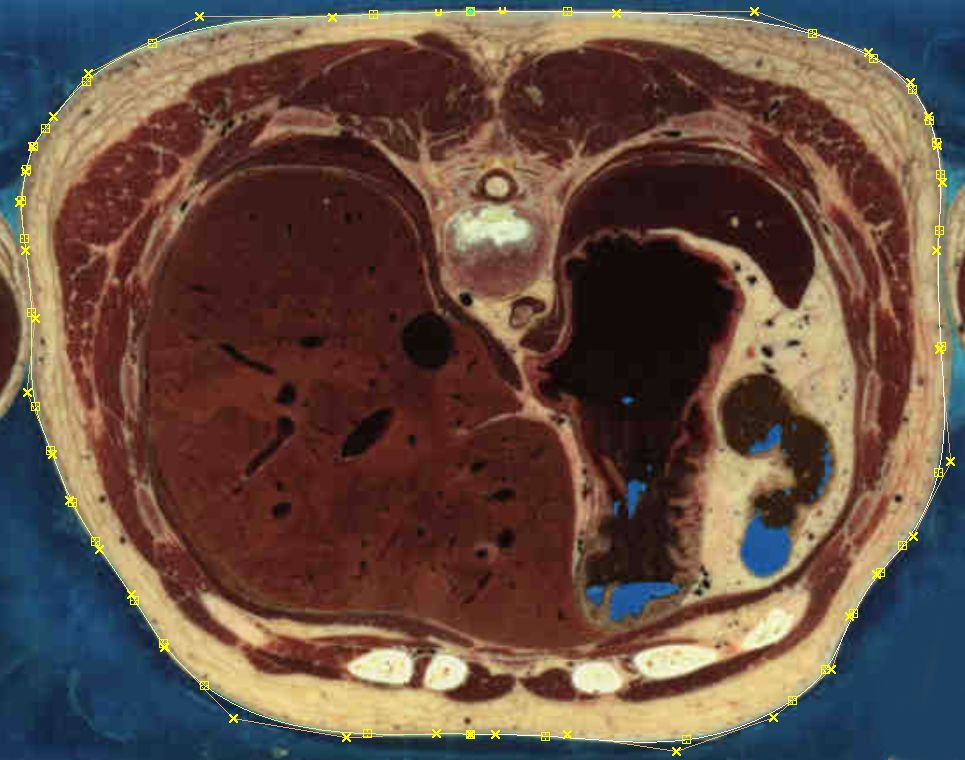
\includegraphics[width= 0.45\textwidth]
         {figures/adult-slice.jpg}
  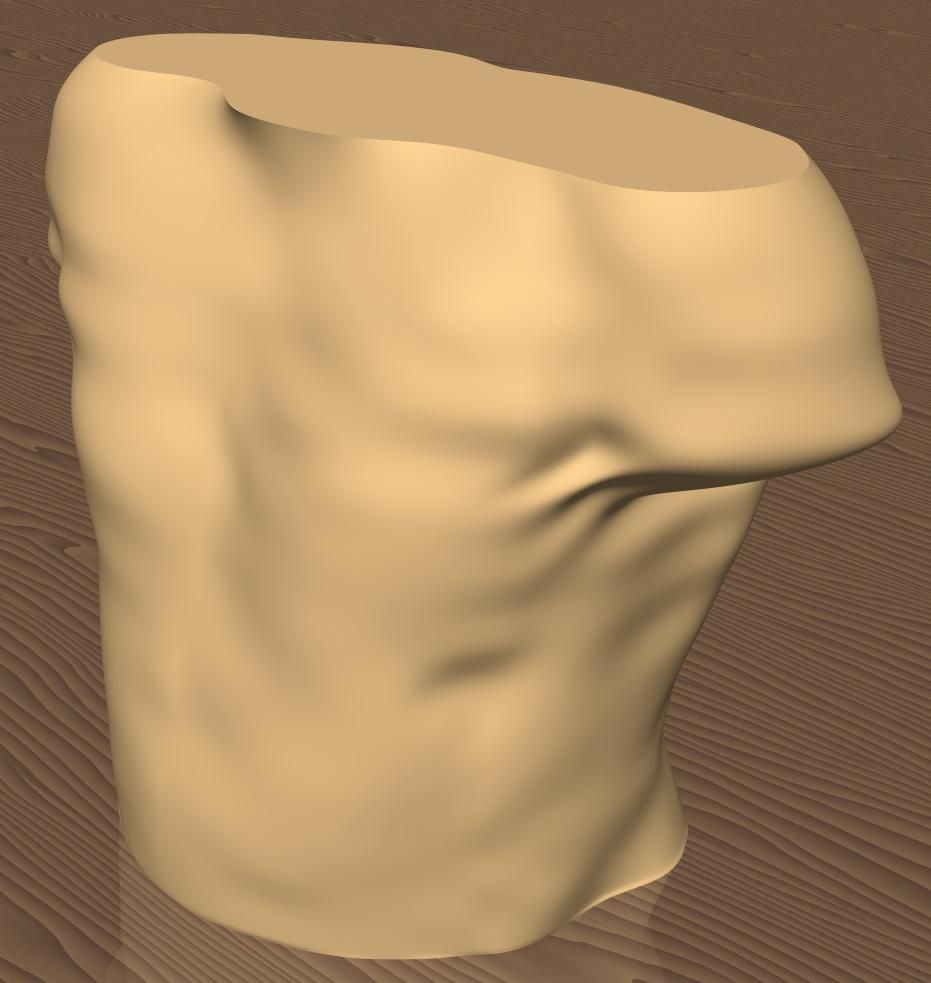
\includegraphics[width= 0.35\textwidth]
         {figures/adult-model.jpg}

\caption{ \label{fig:Adultmodel}
{\em left:} One slice of the male photographic visible body dataset showing the modelled B-Spline curves of the boundary.  There are two curves, modelling the left and right sides of the boundary, tangentially blended.
{\em right:} The finished surface model of the male thorax ready for exporting to the FE meshing software.
}
\end{center}
\end{figure}

The final set of curves are used to generate the body surfaces which are
then capped top and bottom to form a closed volume. The finished surface
model is exported to the mesh-generating software which, in this case,
is I-DEAS (Integrated Design Engineering Analysis Software).
I-DEAS has the tools to define electrode geometry easily prior to meshing,
although any meshing software could be used to achieve this,
e.g. NETGEN (Schoberl 1997).
The meshes generated in I-DEAS were of similar resolution.  The
resulting FEM models are shown in Fig. \ref{fig:AdultFEM}.
For the male, the model comprised 27,170 elements and 5,548 nodes.
For the female, these figures were 27,073 and 5,346 respectively.
These data show that for the male, stretch values were between 0.160
and 0.976, with a mean and SD of 0.698 and 0.109 respectively and for
the female stretch values were between 0.198 and 0.982, with a mean and
SD of 0.702 and 0.101 respectively.

The models generated represent a high degree of accuracy of boundary
shape to a male and female subject.  One limitation is that the
source dataset from the visible
human project was generated from cryogenically frozen cadavers and
will therefore be subject to any anatomical inconsistencies arising from
the process.


\begin{figure}[bhtp]
\begin{center}
  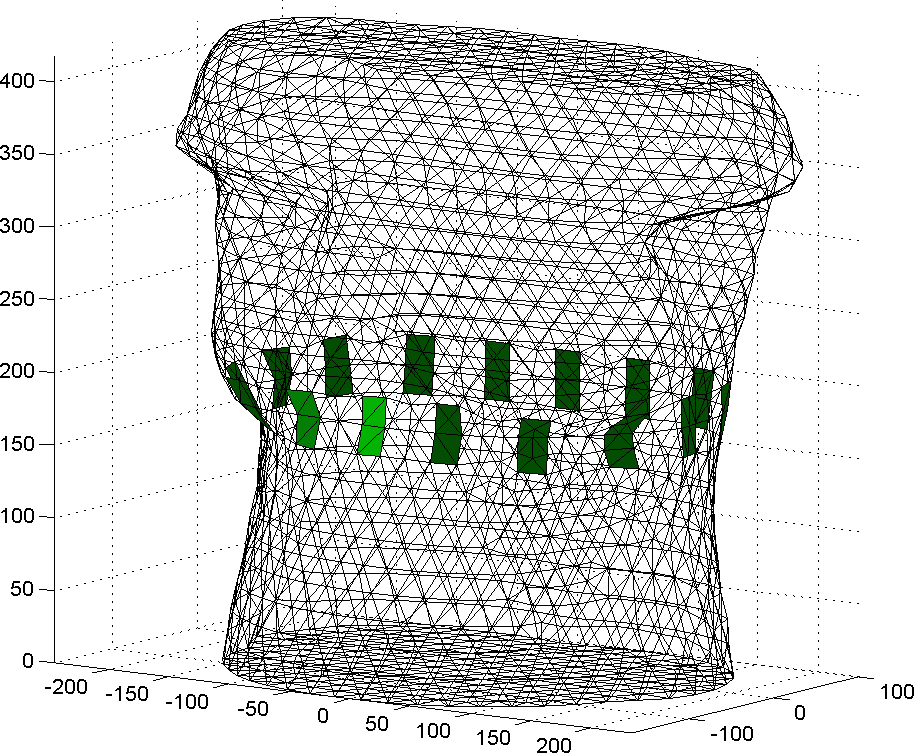
\includegraphics[width= 0.45\textwidth]
         {figures/female_t_mdl.png}
  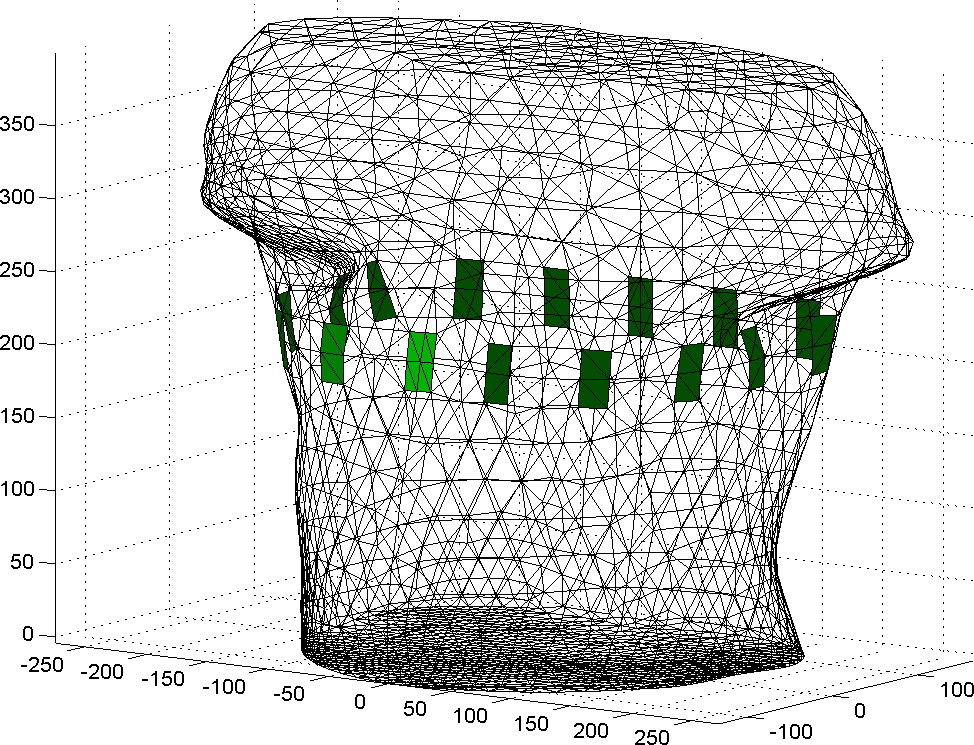
\includegraphics[width= 0.45\textwidth]
         {figures/male_t_mdl.png}
\caption{ \label{fig:AdultFEM}
Finite element models of adult thoraces with
rectangular electrodes. A wire frame mesh
of the surface finite elements is shown.
Electrodes are shown in green,
with a lighter colour electrode \#1.
{\em left:} Female subject
{\em right:} Male subject
}
\end{center}
\end{figure}


\subsection{Neonate models}

The neonatal mesh (Fig.\ \ref{fig:NeonateCyl})
 was generated with the surface modelling
technique used for the adult models. The images 
were from X-Ray CT, based on a 
dataset of an infant with exomphalus. Due to the
risks, CT data of healthy infants are not 
available. The modelling was therefore subject to
some assumptions regarding the boundary shape
of a healthy subject. 
Circular electrodes of 8~mm diameter were specified.
 The model, which
consists of 23,747 elements and 5025 nodes was that used
for initial algorithm evaluation in Bayford et al. (2007).

\begin{figure}[bhtp]
\begin{center}
   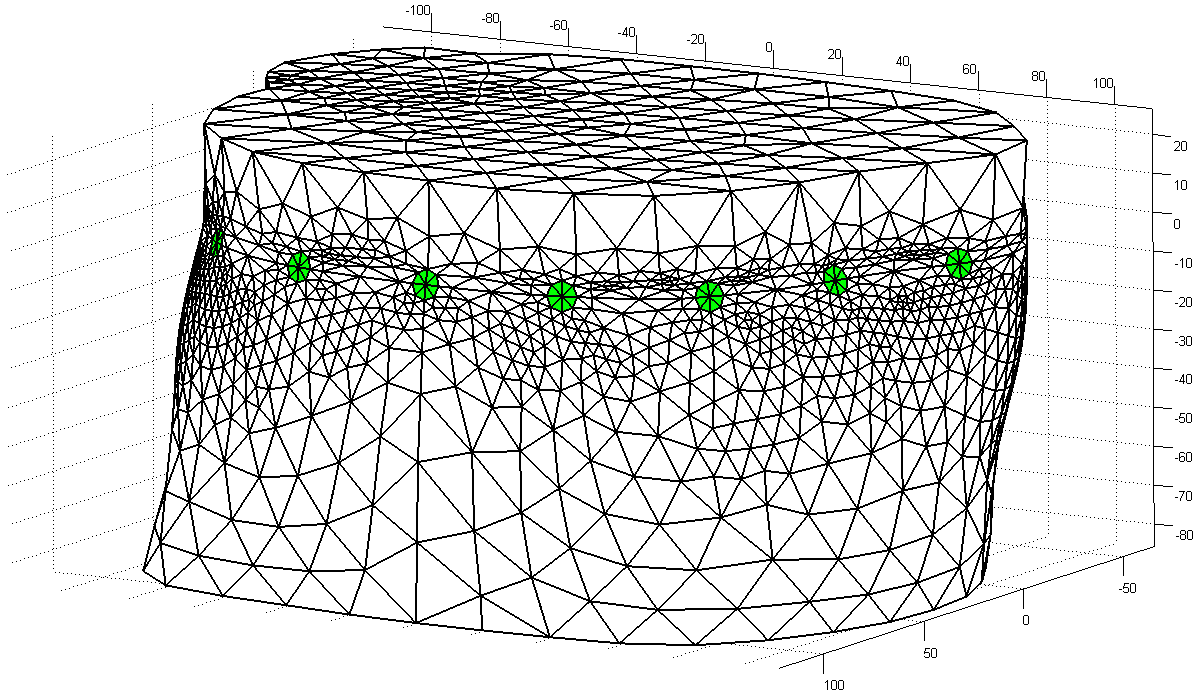
\includegraphics[width= 0.65\textwidth]
         {figures/neonate_t_mdl.png}
  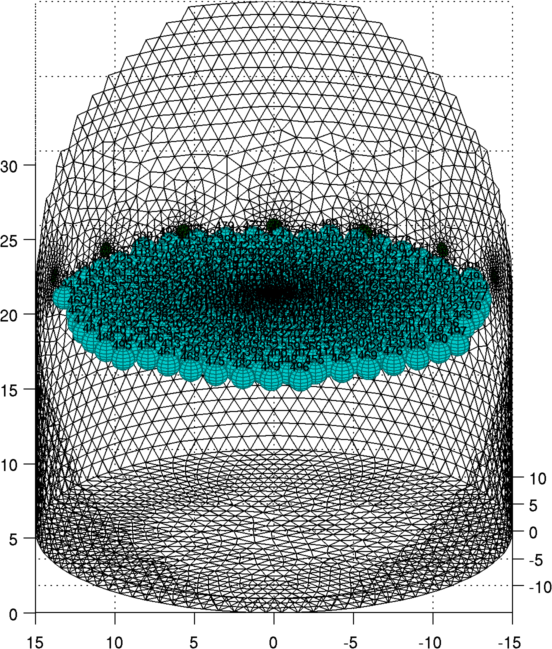
\includegraphics[width= 0.3 \textwidth]
         {../../tutorial/GREIT-evaluation/simulation_3d_test02a.png}
\caption{ \label{fig:NeonateCyl}
%\caption{ \label{fig:NeonateFEM}
%\caption{ \label{fig:CylMesh}
{\em Left:}
Finite element models of a neonatal thorax with
rectangular electrodes. The figure shows a wire frame mesh
of the surface finite elements (in green).
{\em Right:}
Cylindrical FEM used for calculation of the main stimulation
results of this paper. Image shows boundary elements below a cut plane.
The turquoise circles indicate the
positions of conductivity targets, $\xB_t$, used in
sec.\ \ref{sec:perffigm}.
}
\end{center}
\end{figure}


\subsection{Cylindrial models}


A cylindrical FEM model was generated which is suitable for
simulations, phantom tank experiments and is also a reasonable
model for the thorax shape of common EIT experimental animals,
such as pigs.  The FEM is generated using NETGEN (Schoberl, 1997).
The medium diameter
and height are $30$~cm with a maximum element size of $1$~cm.
Circular electrodes are defined by the intersection of the 
main cylinder with radial cylinders, and
electrode mesh refinement is implemented by specifying a
smaller maximum mesh size for each radial cylinder.
Fig.\ \ref{fig:NeonateCyl} shows an image of the resulting
mesh (with 124052 tetrahedral elements) as well as the positions
of conductivity targets.



\section{Evaluation}

Evaluation is performed in two stages. First algorithm performance
is evaluated against the figures or merit in section
\ref{sec:figmerit}.
Next, we compare to a representative set of data
from simulations and experimental.
All evaluation is performed on a 16 electrode EIT configuration
using adjacent current stimulation and voltage measurements.

We compare three algorithms for normalized
difference EIT:
1) Sheffield Backprojection
    ($\RB_{SBP}$), 
2) Gauss-Newton Reconstruction using a
   NOSER prior
    ($\RB_{GN}$), 
and
3) GREIT ($\RB_{GR}$). 
$\RB_{GN}$ is chosen as representative
of typical GN difference EIT solutions.
 In order to normalize
noise performance, each algorithm is set to
NF$=0.5$ at the medium centre. This property
is inherent to the implemented version
of $\RB_{SBP}$. 
For $\RB_{GN}$, NF is set by 
adjusting the hyperparameter $\lambda$, while
for $\RB_{GR}$, NF is set by 
adjusting the weighting $\wB^{(k)}$ of noise
training data $\yB_n$. The value of $\lambda$ is chosen using
a bisection search.


\subsection{Evaluation: performance figures or merit}
\label{sec:perffigm}

\begin{figure}[bhtp]
\begin{center}
\includegraphics[width=0.8\textwidth,
                 bb=0.0in 1.5in 10in 8.0in,page=1]
                {figures/fig-reconst-examples.pdf}
\caption{
\label{fig:FoMimages}
Examples of simulated reconstructed images
({\em red} indicates conductive, while
 {\em blue} indicates non-conductive changes)
 as a function of the simulated target position
({\em left column}, in units of radius fraction). Each row
shows images reconstructed from the same small 
conductivity target, $\xB_t$, shown as 
a small turquoise circle.
{\em left:} Sheffield Backprojection ($\RB_{SBP}$),
{\em center:} Gauss-Newton ($\RB_{GN}$),
{\em right:} GREIT ($\RB_{GN}$).
}
\end{center}
\end{figure}

We test each reconstruction matrix, $\RB$,
for normalized difference EIT
against against the figures of merit 
(sec.\ \ref{sec:figmerit}). Simulation data
are generated from the cylindrical phantom
as shown in Fig.\ \ref{fig:NeonateCyl}. 
Five hundred 
non-conductive targets with a diameter of
5\% of the medium diameter are simulated,
 in the plane of the electrodes,
starting at the medium centre and 
progressing radially outward. The simulated 
target is rotated by a fixed angle around the centre
for each sample in order to sample the entire
FEM geometry.

Fig.\ \ref{fig:FoMimages} shows representative
images at three different radial positions.
Several effects can be seen from these images.
First, Sheffield Backprojection performs well
for targets that are not too close to the 
medium boundary; near the boundary, it produces
smearing artefacts. GN reconstruction produces
clear ringing artefacts, but otherwise shows
good performance with good resolution. 
GREIT gives slightly lower resolution than
GN, but gives more constant resolution with
very little ringing artefacts, matching the
consensus requirements.




\begin{figure}[bhtp]
\begin{center}
  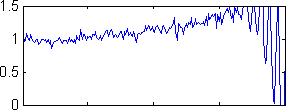
\includegraphics[width= 0.32 \textwidth]
{../../tutorial/GREIT-evaluation/simulation_test_imgs/simulation_test04_12.png}
  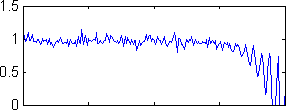
\includegraphics[width= 0.32 \textwidth]
{../../tutorial/GREIT-evaluation/simulation_test_imgs/simulation_test04_22.png}
  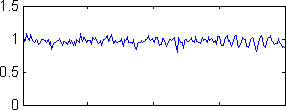
\includegraphics[width= 0.32 \textwidth]
{../../tutorial/GREIT-evaluation/simulation_test_imgs/simulation_test04_42.png}
\put(-420,20){\small AR}
\\
  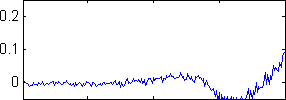
\includegraphics[width= 0.32 \textwidth]
{../../tutorial/GREIT-evaluation/simulation_test_imgs/simulation_test04_13.png}
  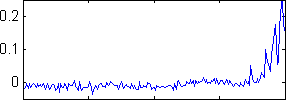
\includegraphics[width= 0.32 \textwidth]
{../../tutorial/GREIT-evaluation/simulation_test_imgs/simulation_test04_23.png}
  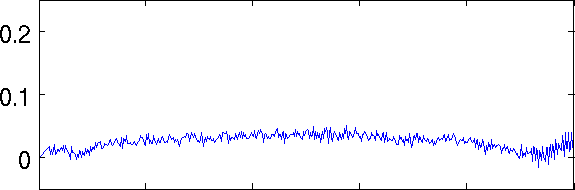
\includegraphics[width= 0.32 \textwidth]
{../../tutorial/GREIT-evaluation/simulation_test_imgs/simulation_test04_43.png}
\put(-420,20){\small PE}
\\
  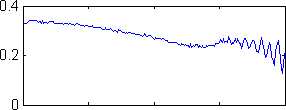
\includegraphics[width= 0.32 \textwidth]
{../../tutorial/GREIT-evaluation/simulation_test_imgs/simulation_test04_14.png}
  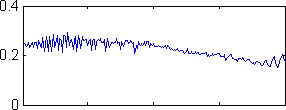
\includegraphics[width= 0.32 \textwidth]
{../../tutorial/GREIT-evaluation/simulation_test_imgs/simulation_test04_24.png}
  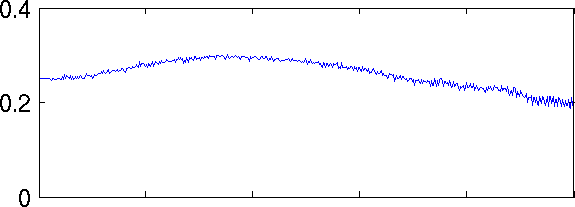
\includegraphics[width= 0.32 \textwidth]
{../../tutorial/GREIT-evaluation/simulation_test_imgs/simulation_test04_44.png}
\put(-420,20){\small RES}
\\
  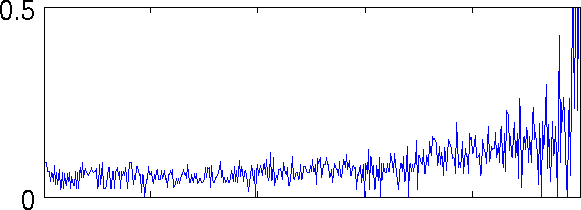
\includegraphics[width= 0.32 \textwidth]
{../../tutorial/GREIT-evaluation/simulation_test_imgs/simulation_test04_15.png}
  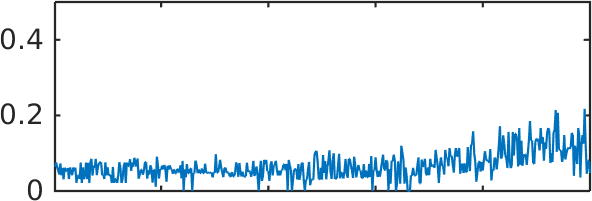
\includegraphics[width= 0.32 \textwidth]
{../../tutorial/GREIT-evaluation/simulation_test_imgs/simulation_test04_25.png}
  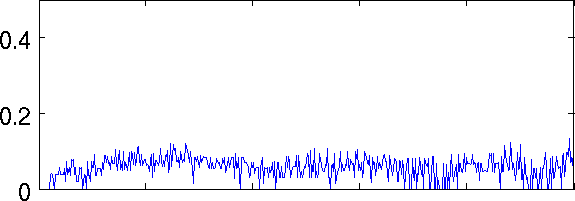
\includegraphics[width= 0.32 \textwidth]
{../../tutorial/GREIT-evaluation/simulation_test_imgs/simulation_test04_45.png}
\put(-420,20){\small SD}
\\
  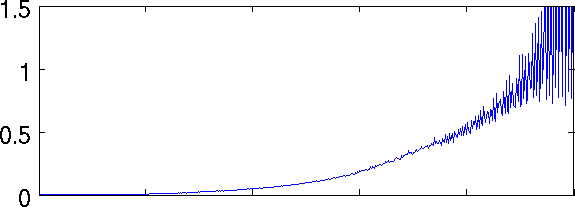
\includegraphics[width= 0.32 \textwidth]
{../../tutorial/GREIT-evaluation/simulation_test_imgs/simulation_test04_16.png}
  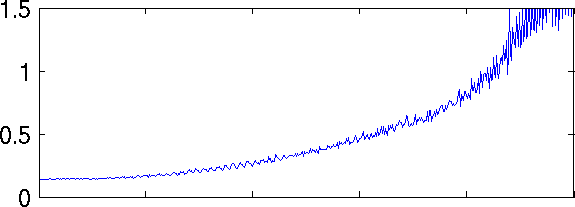
\includegraphics[width= 0.32 \textwidth]
{../../tutorial/GREIT-evaluation/simulation_test_imgs/simulation_test04_26.png}
  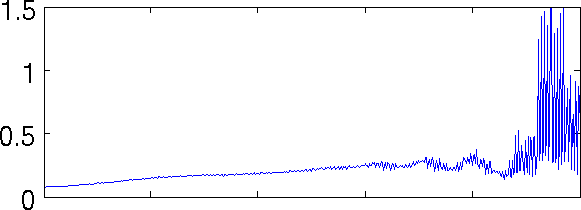
\includegraphics[width= 0.32 \textwidth]
{../../tutorial/GREIT-evaluation/simulation_test_imgs/simulation_test04_46.png}
\put(-420,20){\small RNG}
\caption{ \label{fig:FoMresults}
Algorithm performance against simulated tests as a function
of radial position. Radial position on each graph is
from centre ({\em left}) to the body boundary ({\em right}).
Each column shows results from a different reconstuction
algorithm:
{\em left:} Sheffield Backprojection ($\RB_{SBP}$),
{\em center:} Gauss-Newton ($\RB_{GN}$)
{\em right:} GREIT ($\RB_{GR}$)
Each row shows a different parameter. From
top to bottom: 
Amplitude Response (AR),
Position Error (PE),
Resolution (RES),
Shape Deformation (SD) and 
Ringing (RNG)
}
\end{center}
\end{figure}

Fig.\ \ref{fig:FoMresults} shows algorithm performance
for each parameter as a function of radial position.
The ``noise'' that appears on each line is due to the
discreteness of the FEM mesh for simulation. 
There are larger oscillations
near the boundary; this reflects variability in 
performance as the target passes in front of and
between the electrodes.
Overall, all algorithms perform well
in the centre of the medium with poorer performance
near the boundary. In comparison to
SBP and GN, GREIT shows either an equivalent or an improved
ability to meet the desired
performance requirements.


\subsection{Evaluation: representative data}

In order to illustrate EIT image reconstructions
with these algorithms, we calculate images using
$\RB_{SBP}, \RB_{GN}, {\rm and~}\RB_{GR}$
for two experiments in which the physiology 
corresponding to the EIT images is well understood.
Due to space constraints, other tests of GREIT
are given on the internet at \verb+eidors.org/GREIT+. 

\begin{itemize}
%\item
%{\em Experimental lung injury:}
%These data were measured in anesthetized
%ventilated supine pigs as part of the study of
%Frerichs \etal  (1998) using the 
%Sheffield MK I EIT system. EIT measurements
%were made on the initially healthy animals.
%Subsequently, oleic acid was applied 
%into the left pulmonary artery to produce
%selective unilateral lung injury, and new 
%EIT measurements were taken.  
%Images are reconstructed of tidal ventilation
%in a pig before and after unilateral lung
%injury. Measurements $\vB_r$ and $\vB$
%were calculated from average end-expiratory
%and end-inspiratory measurements, respectively.
%
%\begin{figure}[bhtp]
%\begin{center}
%%\includegraphics[width=0.8\textwidth,
%\caption{
%\label{fig:Frerichs98images}
%Images of ventilation in a pigs shown ({\em top row})
%before and ({\em bottom row}) after unilateral
%lung injury (data from Frerichs \etal 1998).
%Images are shown for three algorithms.
%{\em left:} Sheffield Backprojection ($\RB_{SBP}$),
%{\em center:} Gauss-Newton ($\RB_{GN}$),
%{\em right:} GREIT ($\RB_{GN}$).
%}
%\end{center}
%\end{figure}
%
\item
{\em Recruitment manoeuvre in acute lung injury:}
These data were measured in an anesthetized
ventilated supine piglet as part of the study of
Frerichs \etal  (2003) using the 
Goe MF II system, and performed at the
University of G\"ottingen, Germany. Acute lung injury
was created by repeated
bronchoalveolar lavage. EIT data were
measured during a recruitment manoeuvre
during which PEEP was raised and then
lowered from 0 to 30~cmH$_2$O in steps. 
Images are reconstructed of tidal ventilation
at a PEEP of $10$~cmH$_2$O on the inflation
and deflation segments of a recruitment manoeuvre.
Measurements $\vB_r$ and $\vB$
were calculated from average end-expiratory
and end-inspiratory measurements at the specified
PEEP.

\begin{figure}[bhtp]
\begin{center}
\includegraphics[width=0.20\textwidth]{figures/example_images_111.png}
\includegraphics[width=0.20\textwidth]{figures/example_images_211.png}
\includegraphics[width=0.20\textwidth]{figures/example_images_411.png}
\\
\includegraphics[width=0.20\textwidth]{figures/example_images_112.png}
\includegraphics[width=0.20\textwidth]{figures/example_images_212.png}
\includegraphics[width=0.20\textwidth]{figures/example_images_412.png}
\caption{
\label{fig:Frerichs03images}
Images of ventilation in a pig with
acute lung injury 
at a PEEP of $10$~cmH$_2$O shown ({\em top row})
on the inflation and ({\em bottom row})
deflation segment of a stepwise recruitment and derecruitment manoeuvre 
(data from Frerichs \etal 2003).
{\em left:} GREIT ($\RB_{GN}$).
{\em center:} Gauss-Newton ($\RB_{GN}$),
{\em right:} Sheffield Backprojection ($\RB_{SBP}$),
}
\end{center}
\end{figure}

\item
{\em Regional pneumothorax / pleural effusion:}
These data were measured in anesthetized
ventilated supine pigs as part of the
study of Hahn \etal (2006) using the
Goe MF II EIT system and performed at the
University of G\"ottingen, Germany.
Unilateral pleural effusion and pneumothorax was
induced by injecting up to $300$~ml of air or $300$~ml of
Ringer solution into the right side via a small incision
made in the chest wall and a plastic canula and
fixed by a suture and sealed by cyanoacrylate glue.
Images are reconstructed of pneumothorax
and pleural effusion.
Measurement $\vB_r$ is calculated from an
average signal at end-expiration before
the intervention, while $\vB$ is calculated
at end-expiration during injection of air
and fluid, respectively.

\begin{figure}[bhtp]
\begin{center}
\includegraphics[width=0.20\textwidth]{figures/example_images_115.png}
\includegraphics[width=0.20\textwidth]{figures/example_images_215.png}
\includegraphics[width=0.20\textwidth]{figures/example_images_415.png}
\\
\includegraphics[width=0.20\textwidth]{figures/example_images_116.png}
\includegraphics[width=0.20\textwidth]{figures/example_images_216.png}
\includegraphics[width=0.20\textwidth]{figures/example_images_416.png}
\caption{
\label{fig:Frerichs98images}
Images of localized
({\em top row})
pneumothorax, and
({\em bottom row})
pleural effusion
in an anesthetized, ventilated pig 
(data from Hahn \etal 2006).
{\em left:} GREIT ($\RB_{GN}$).
{\em center:} Gauss-Newton ($\RB_{GN}$),
{\em right:} Sheffield Backprojection ($\RB_{SBP}$),
}
\end{center}
\end{figure}


\end{itemize}


\section{Discussion}

This paper describes a unified approach to 2D linear EIT
reconstruction of lung images, which we call GREIT.
This approach represents
a consensus of a large and representative
group of experts in EIT algorithm design and clinical
applications for pulmonary monitoring. The goal of
this work is to address the concern that most
clinical and physiological research in lung EIT
is done using older and proprietary algorithms, which is
an obstacle to interpretation of EIT images because the
reconstructed images are not well characterized.

The approach consists of:
1) detailed 3D finite element models of the thorax;
2) consensus on the performance figures of merit;
and
3) an approach to fit the linear reconstruction
 matrix, $\RB$, to the performance figures.
In order of importance, figures of merit are:
a) uniform amplitude response,
b) small and uniform position error,
c) small ringing artefacts,
d) uniform resolution,
e) limited shape deformation, and
f) high resolution.
Such figures of merit are to be achieved with
small noise amplification and
small sensitivity to electrode and boundary movement.
The current work leaves several parameters of the algorithm
unspecified, including details on the selection of training
data and required noise parameters. We are currently undertaking
clinical and experimental validation of the GREIT algorithm
to establish recommendations for these parameters.
It is worth clarifying one disadvantage of the regularized
approach presented: Sheffield backprojection tend to map
measurement artefacts to ``streaks'', while GREIT maps the same
artefacts to ``blobs''. It is easier for an operator to notice
such streaks, and identify the presence of data errors.

All contributions from this work
(algorithms, software, models and test data)
 have been made available (\verb+eidors.org/GREIT+) 
under an open source license which allows
gratis commercial and non-commercial use.
Software to implement this algorithm is made
available under the GNU LGPL (Free Software Foundation, 2007),
which requires the source code of any distributed
 modifications to be made available.
FEM models, GREIT reconstruction matrices ($\RB_{GR}$) and
experimental and clinical data provided for evaluation of GREIT,
are made available under the Creative Commons Attribution
License (Creative Commons, 2007). Users are permitted
to copy, distribute, transmit and adapt the works,
under the condition of attribution by citing the
papers as indicated.



\References % Harvard style references
\item[]
Adler A and Guardo R 1996 Electrical impedance tomography:
regularized imaging and contrast detection {\em IEEE Trans. Med.
Imaging} {\bf 15} 170-179

\item[]
Adler A, Guardo R and Berthiaume Y 1996 Impedance imaging of lung
ventilation: Do we need to account for chest expansion? {\em IEEE
Trans. Biomed. Eng.} {\bf 43}(4) 414-20


\item[]
Adler A and Lionheart W R B 2006
``Uses and abuses of EIDORS: An extensible software base for EIT''
{\em Physiol Meas}
27 S25--S42

\item[]
Ackerman M J  1998  
The Visible Human Project
{\em Proc. IEEE}
86 504--511


%\item[]
%Barber D C
%Brown B H
%Freeston I L, 1983
%Imaging spatial distributions of resistivity using applied potential tomography
%{\em Electronics Letters}
%19 933--935
%

\item[]
Barber D C and Brown B H 1984
``Applied potential tomography'', 
{\em J Phys E: Sci Instrum}
 17 723--733

\item[]
Barber D C and Brown B H 1988 Errors in reconstruction of
resistivity images using a linear reconstruction technique {\em
Clin. Phys. Physiol. Meas.} 
9(suppl. A) 101--4

\item[]
Barber D C 1989
``A review of image reconstruction techniques for electrical
 impedance tomography''
{\em Med Phys}
16 162--169

\item[]
Bayford R H Kantartzis P Tizzard A Yerworth R Liatsis P and Demosthenous A
 2008
Development of a neonate lung reconstruction algorithm using a wavelet
 AMG and estimated boundary form
{\em  Physiol Meas} 29 S125--S138.


\item[]
Brown B H and Seagar A D 1987 
``The Sheffield data collection system''
{\em Clin Phys Physiol Meas}
 8(Suppl A) 91--97

\item[]
Brown B W 2003
``Electrical impedance tomography (EIT): a review''
{\em J Medical Eng. \& Technology}
27 97--108


\item[]
Cheney M, Isaacson D, Newell J C, Simske S and Goble J C 1990
NOSER: an algorithm for solving the inverse conductivity problem
{\em Int.J.Imaging Syst.Technol.} 
2 66--75

\item[]
Cheng KS, Newell JC, Gisser DG, 1989
"Electrode Models for Electric Current Computed Tomography"
{\em IEEE Trans. in Biomedical Eng.}
36 918--924


\item[]
Cohen-Bacrie C  Goussard Y and Guardo R
1997
Regularized Re construction in Electrical
Impedance Tomography Using a Variance
Uniformization Constraint 
{\em IEEE Trans. Med. Imag.} 16 562-571

\item[]
Coulombe N, Gagnon H, Marquis F, Skrobik Y, Guardo R, 2005
A parametric model of the relationship between EIT and total lung volume
{\em Physiol. Meas.}
26 401--411


\item[]
Creative Commons/Science Commons 2007
``Creative Commons 3.0 Attribution License''
\verb+creativecommons.org/licenses/by/3.0/+

%\item[]
%Frerichs I  Hahn G Schr\"oder T Hellige G 1998
%Electrical impedance tomography in
%monitoring experimental lung injury
%{\em Intensive Care Med.}
%24 829--836
%
\item[]
Frerichs I Dargavillle P A Dudykevych T Rimensberger P M 2003
Electrical Impedance Tomography - a method for monitoring
regional lung aeration and tidal volume distribution?
{\em  Intensive Care Med.}
29 2312--2316

\item[]
GNU Lesser General Public License: Version 3, 29 June 2007
{\em Free Software Foundation, Inc.}
\verb+www.gnu.org/licenses/lgpl.html+

G\'omez-Laberge C Adler A 2008
Direct EIT Jacobian calculations for conductivity change and electrode movement
{\em Physiol. Meas.}
29 S89--S99


% \item[]
% Hahn G Thiel F Dudykevych T Frerichs I Gersing E
% and Hellige G 2001
% ``Quantitative evaluation of the performance of
% different electrical tomography devices''
% {\em  Biomed Tech (Berl)}
% 46 91--95

\item[]
Hahn G, Dudykevych T, Frerichs I, Thiel F and Hellige G 2002
A high performance electrical impedance tomography
(EIT) system for clinical evaluation studies and space application
{\em Proc. Conf. 2nd European Medical and
Biol Eng} Vienna, Austria 110--111

\item[]
Hahn G Just A Dudykevych T Frerichs I Hinz J  Quintel M Hellige G
2006
Imaging pathologic pulmonary air and fluid accumulation by
 functional and absolute EIT
{\em Physiol. Meas.}
27 S187--S198

\item[]
Hahn G Just A Dittmar J  Hellige G 2008
Systematic errors of EIT systems determined by easily-scalable
 resistive phantoms
{\em Physiol. Meas.}
 29 S163--S172



\item[]
Hartinger A E Gagnon H Guardo R 2007
Accounting for Hardware Imperfections in EIT Image
Reconstruction Algorithms.
{\em Physiol. Meas.}
28 13--S27
 
\item[]
Lionheart W R B 2004
EIT reconstruction algorithms: pitfalls, challenges
and recent developments
{\em Physiol. Meas.}
25 125--142

\item[]
Oh S, Tang T, Sadleir R 2007
Quantitative analysis of shape change in Electrical Impedance Tomography (EIT)
in {\em IFMBE Proceedings}
17 424--427

\item[]
Polydorides N and Lionheart W R B 2002 A Matlab toolkit for
three-dimensional electrical impedance tomography: A contribution
to the Electrical Impedance and Diffuse Optical Reconstruction
Software project {\em Meas. Sci. Technol.} {\bf 13} 1871-83

\item[]
Santosa F Vogelius M 1990
Backprojection algorithm for electrical impedance imaging
{\em SIAM J. Applied Math}
50 216--243. 

\item[]
Schoberl J 1997
NETGEN: An advancing front 2D/3D-mesh generator based on abstract rules
{\em Computing and Visualization in Science}
1 41--52 

\item[]
Smit H J
Vonk Noordegraaf A
Marcus R
Boonstra A
de Vries P M 
Postmus P E
2004
Determinants of pulmonary perfusion measured by electrical impedance tomography
{\em Eur. J. Appl. Physiol.}
92 45--49

\item[]
Soleimani M, G\'omez-Laberge C and Adler A 2006 Imaging of
conductivity changes and electrode movement in EIT \PM {\bf 27}
S103--S13

\item[]
Tizzard A Horesh L Yerworth R J Holder D S Bayford R H 2005
Generating accurate finite element meshes for the forward
model of the human head in EIT
{\em Physiol. Meas.}
 26 S251--61 

\item[]
Vauhkonen M, Vad\`asz D, Karjalainen P A, Somersalo E and
Kaipio J P 1998
 Tikhonov regularization and prior information in
electrical impedance tomography
 {\em IEEE Trans Med Imaging}
17 285--93

\item[]
Victorino JA, Borges JB, Okamoto VN, Matos GF, Tucci MR, Caramez MP, Tanaka H, Sipmann FS, Santos DC, Barbas CS, Carvalho CR, Amato MB 2004
Imbalances in regional lung ventilation: a validation study on
electrical impedance tomography.
{\em Am J Respir Crit Care Med} 169:791--800

\item[]
Wheeler JL, Wang W, Tang M 2002
A comparison of methods for measurement of spatial resolution in two-dimensional circular EIT images
{\em Physiol. Meas.}
23 169--176

\item[]
Wolf GK, Grychtol B, van Genderingen H, Zurakowski D, Thompson JE, Arnold JH
2007.
Regional lung volume changes in children with acute respiratory distress
syndrome during a derecruitment maneuver
{\em Crit Care Med}
35 1972--1978.

\item[]
Yang F  Patterson R 2007
The contribution of the lungs to thoracic impedance
measurements: a simulation study based on a high
resolution finite difference model
{\em Physiol. Meas.}
28 S153--S163

\item[]
Yorkey T J, Webster J G and Tompkins W J 1987
Comparing reconstruction algorithms for electrical
impedance tomography
{\em IEEE Trans. Biomed. Eng}
34 843--52


\item[]
Zhang J and Patterson R P 2005 EIT images of ventilation: what
contributes to the resistivity changes?
{\em Physiol. Meas.}
 26 S81--S92

\endrefs

\end{document}
